%!TEX program = xelatex
% 完整编译: xelatex -> biber/bibtex -> xelatex -> xelatex
\documentclass[lang=cn,11pt,a4paper]{elegantpaper}

\title{Poisson.h文档说明}
\author{Haochen Huang}
\institute{西安交通大学MFM课题组}

\version{4.02test}
\date{\zhtoday}


% 本文档命令
\usepackage{array}

\begin{document}

\maketitle
\tableofcontents

\begin{abstract}
本文为basilisk的头文件Poisson.h的说明文档。\par
2.02更新:更新模板添加高亮、索引,更新文章内容,修正某些显示错误并添加程序结构图及说明。\par
3.02更新:更正$relax$函数中$Jacobi$与$GS$迭代之间的关系,回顾之前相关使用函数指针进行输入的地方,指出改装求解器的可能条件。\par
4.02更新:添加不同层级网格迭代的相应细节,添加Basilisk网格的判定方式及相应数据点的插值方法。
\end{abstract}

\section{理论背景}
相关细节参考Basilisk原作者著作\cite{popinet2003gerris}\cite{popinet2015quadtree}
\subsection{Poisson方程由来}
我们可以由bcg.h中的对流方程求出一个速度场$U^{**}$,由于速度物理特性,其必然是光滑且连续的,由Hodge分解可得,该速度场可以分为一个无散场与无旋场即:
\begin{equation}
    U^{**} = U + \nabla \phi
\end{equation}
其中$\nabla U = 0$这样$U$就既满足动量方程又满足不可压方程,为真实速度解。
\subsection{Relaxation函数由来}
求解Poisson方程
\begin{equation}
    \nabla^2 \phi = \nabla U^{**}
\end{equation}
针对某一个单元,在单元内部对上式进行体积分有:
\begin{equation}
    \int_{\partial \mathscr{B}}\nabla \phi \cdot \mathbf{n} = \int_{\mathscr{B}}\nabla U^{**}
\end{equation}
在单元上进行离散有:
\begin{equation}
    \sum_d h\nabla_d \phi =h^2 \nabla \cdot U^{**}
\end{equation}
其中下角标$d$表示方向,在离散过程中等式左边数据储存于单元面中心,而等式右边则是单元体中心。在bcg.h中我们已经利用已知的$u^n$将$U^{**}$计算出来了,现在的目标则是计算$\phi$。\par
为了得到$\phi$,我们假设$\phi$在单元表面上的梯度值$\nabla_d \phi$可以用在单元中心的$\phi$线性表示,即:
\begin{equation}
    \nabla_d \phi = \alpha_d \phi + \beta_d
\end{equation}
其中$\alpha, \beta$均为常数,其值根据周边网格情况等可以计算出来,暂时按下不表。由此我们可以得到相应$\phi$值表达式
\begin{equation}
    \sum_d h\nabla_d \phi = \sum_d\alpha_d\phi + \sum_d\beta_d
\end{equation}
即有:
\begin{equation}
    \mathscr{R}(\phi, \nabla U^{**})=\phi \leftarrow \frac{h\nabla\cdot U^{**}-\sum_d\beta_d}{\sum_d\alpha_d}
\end{equation}
即能够构成$\mathscr{L}(A) = B$的$A,B$都可以满足Relaxation函数关系。
\subsection{Jacobi迭代}
在构建完Relaxation函数后,我们将对其使用Jacobi迭代,以完成相应求解。\par
假设我们有方程组
\begin{align}
    a_{11}x_1+a_{12}x_2+\cdots+a_{1n}x_n & =b_1\notag\\
    a_{11}x_1+a_{22}x_2+\cdots+a_{2n}x_n & =b_2\\
    \vdots \quad \vdots \quad& \vdots\notag \\
    a_{n1}x_1+a_{n2}x_2+\cdots+a_{nn}x_n & =b_n\notag
\end{align}
不考虑收敛问题,我们将$\mathbf{x}^0={x_1^0,x_2^0\cdots x_n^0}$依次带入方程求解得到$\mathbf{x}^1={x_1^1,x_2^1\cdots x_n^1}$,依次迭代,依据相应理论,在迭代次数足够多的情况下,解最终会收敛于方程真解。\par
根据之前构建的Relaxation函数,由于$\nabla U^{**}$已知,我们可以对场量$\phi$采取类似的迭代方式,最终得到目的解。
\section{具体算法}
$\mathscr{L}$为线性算子即:
\begin{equation}
    \mathscr{L}(\phi+\delta \phi) =\mathscr{L}(\phi)+\mathscr{\delta \phi} 
\end{equation}
其中$\mathscr{L}(\phi+\delta\phi)=\nabla U^{**}$而$\phi$为预测值,那么$\delta \phi$就是预测值与真实值之差,令残差$R$为
\begin{equation}
    R = \nabla U^{**} - \mathscr{L}(\phi)
\end{equation}
由此$\delta \phi$与$R$构成了拉普拉斯算对,他们之间的关系就可以用Relaxation函数$\mathscr{R}$来表示。\par
接下来介绍Basilisk的自适应网格模式。\par
\begin{figure}[h]
  \centering
  \includegraphics[height=5.5cm]{wangge.png}
  \caption{二维情况下,同一单元网格级别变化情况,摘自\cite{popinet2003gerris}}\label{fig:wangge}
\end{figure}
如图\ref{fig:wangge}中所示,其中$Ml$表示网格加密级别;注意,这是同一个网格的不同加密形式。
$l$层的残差可以由$l+11$计算得出即
\begin{equation}
    R_l=\frac{\sum_i h^2R_{l+1}}{\sum_i h^2}
\end{equation}
\begin{algorithm}[t]
    \caption{Poisson solver框架}
	\label{alg:algorithm1}
	\KwIn{初始$\phi^0$,最密网格$M_L$}
	\KwOut{相应计算区域中全场$\phi$值}  
	\BlankLine
	由$\phi^0$计算再$M_L$上的残差$R_L$
	
	\While{\textnormal{$\left|\alpha R_L\right|_{\infty}<\epsilon$}}
	{
		\For{$l=L-1;l\geq0;l--$}
		{
		    由$R_{l+1}$计算$R_l$;\\
		}
		在最低级网格$M_0$上使用$\mathscr{R}(\delta \phi,R_0)$直到最后的值收敛;\\
		\For{$l=1;l\leq L; l++$}
		{
		    将在$M_{l-1}$上获得的$\delta \phi$在空间上进行插值后直接作为初始猜测值进行$\mathscr{R}(\delta \phi, R_l)$的$n$次迭代;\\
	    }
	    将迭代计算出的$\delta \phi$附加在原本$M_L$的$\phi$值上;\\
	    再次计算$R_L$;\\
	}
	return $\phi$;\\
\end{algorithm}

\section{源代码解析}
\subsection{源代码构成及结构简介}
Poisson.h主要求解的方程为广义的Poisson–Helmholtz即:
\begin{equation}\label{equ:L}
    L(a) = \nabla\cdot (\alpha\nabla a)+\lambda a=b
\end{equation}
源代码一共分为四个部分,分别是:
\begin{enumerate}
    \item Multigrid cycle函数的构建\ref{sec:multicycle},此函数表示算法中的第二个for循环,即在已知各个级别网格的残差后,通过$\mathscr{R}$函数进行迭代,并向高一层级网格进行差分,得到该网格$\delta a$的初始值,该函数并没有$\mathscr{R}$的定义
    \item Multigrid solver函数构建\ref{sec:multisolver},该函数与Multigrid cycle函数一同构成完整的算法循环框架(Multigrid cycle 将会在其中被引用),该函数负责判断计算域内的最大残差是否满足标准,以及当某些限定情况发生时,对迭代次数进行改变
    \item 两个重要功能函数的构建\ref{sec:relaxres}:$relax$函数即$\mathscr{R}$,以及计算残差的residual函数,这两个函数在之前构建的整体框架中均被引用。
    \item 整体合并解决问题的示例\ref{sec:example}
\end{enumerate}
其相互关系如下图所示:
\begin{figure}[h]
  \centering
  \includegraphics[scale=0.3]{poisson.png}
  \caption{poisson.h头文件中主要函数关系}
\end{figure}
由图所示,mg solver为求解器的主体部分,其主要功能在于调配各个函数的调用顺序,判断是否满足输出标准,以及调整循环的次数,而$mg\,cycle$与$relax$函数则构成了一次或数次(基于$mg\,solver$传入参数调控)完整的G-S迭代,并更新初始值,并将结果传递至$residual$计算残差,$residual$返回残差供$mg\,solver$进行判断,选择调整参数再次进入循环或者跳出循环输出结果。
\subsection{Multigrid cycle函数}\label{sec:multicycle}
函数输入计算目标指针$a$,残差指针$res$,修正目标值指针$da$,以及$\mathscr{R}$函数指针$relax$等进行从最低层级向最高层级网格的残差修正。\par
注意此处输入值中包含函数指针,修改者可以通过传入具有相同参变量的函数达到改装求解器的目的。
\begin{minted}[mathescape=true,breaklines]{lexer.py:DiffLexer -x}
void mg_cycle (scalar * a, scalar * res, scalar * da,
           void (* relax) (scalar * da, scalar * res, 
                int depth, void * data),
           void * data,
           int nrelax, int minlevel, int maxlevel)
{
  restriction (res);//利用平均计算每一层级网格上残差值
  
  //从最低的网格密度层级开始对相应的计算区域进行Jacobi迭代
  minlevel = min (minlevel, maxlevel);
  for (int l = minlevel; l <= maxlevel; l++) {

    if (l == minlevel)
      foreach_level_or_leaf (l)//对当前级别网格,或小于l级但已经是leaf的网格进行遍历
        for (scalar s in da)
            foreach_blockf (s)//默认在common.h中定义为空,具体定义在grid/layers.h中,用法应该与存储数据方式相关,用于快速遍历内存上值,测验后发现其存在对结果并没有影响
                s[] = 0.;
    else
      foreach_level (l)
        for (scalar s in da)
            foreach_blockf (s)
                s[] = bilinear (point, s);
    //在轮到$l$级网格时,由于网格加密导致网格中心位置变动,需要对上一级中求出的$da$进行插值,并将其作为本轮Jacobi迭代的初始值
    
    boundary_level (da, l);
    for (int i = 0; i < nrelax; i++) {
      relax (da, res, l, data); //利用$\mathscr{R}$函数进行Jacobi迭代,迭代次数为输入值nrelax,该数值在后面会视情况而改变。
      boundary_level (da, l);
    }
  }

  foreach() {
    scalar s, ds;
    for (s, ds in a, da)
      foreach_blockf (s)
        s[] += ds[];//更新最密网格中的目标数值$a$
  }
}

\end{minted}
由此,算法中的Jacobi迭代进行完毕。
\subsection{Multigrid solver函数}\label{sec:multisolver}
该函数通过在其中通过引用$Multigrid\,cycle$构建完整的算法结构,
其首先定义两种数据结构,首先是表示整个计算域状态的数据结构$mgstats$:
\begin{minted}[mathescape=true,breaklines]{lexer.py:DiffLexer -x}
int NITERMAX = 100, NITERMIN = 1;
double TOLERANCE = 1e-3;//默认定义,包括迭代次数与残差宽容度

typedef struct {
  int i;              // 总循环次数
  double resb, resa;  // 在迭代前后残差的最大值,用于结束循环判断
  double sum;         // sum of r.h.s.(r.h.s.代表等式右端,即所有的b的和)
  int nrelax;         // Jacobi循环$\mathscr{R}$次数
  int minlevel;       // 网格密度的最低密度等级
} mgstats;
\end{minted}
以及所需要求解目标函数的数据结构:
\begin{minted}[mathescape=true,breaklines]{lexer.py:DiffLexer -x}
struct MGSolve {
  scalar * a, * b;
  double (* residual) (scalar * a, scalar * b, scalar * res,
               void * data);// 求解残差的函数,在下一节会出现
  void (* relax) (scalar * da, scalar * res, int depth, 
          void * data);
  void * data;// 该参数的具体细节将在下一节展示
  
  int nrelax;
  scalar * res;
  int minlevel;
  double tolerance;
};
\end{minted}
我们构成的函数mg$\underline{~}$solve返回值的数据类型为mgstats即循环状态,输入值则为MGSlove型数据$p$
\begin{minted}[mathescape=true,breaklines]{lexer.py:DiffLexer -x}
mgstats mg_solve (struct MGSolve p)
{
  //根据输入数据格式的$a$分配修正数据的指针,即保证$da$与其有相同的分布与边界条件
  scalar * da = list_clone (p.a), * res = p.res;
  if (!res)
    res = list_clone (p.b);

  /**
  The boundary conditions for the correction fields are the
  *homogeneous* equivalent of the boundary conditions applied to
  *a*. */

  for (int b = 0; b < nboundary; b++)
    for (scalar s in da)
      s.boundary[b] = s.boundary_homogeneous[b];
  
  // $s$即为要返回的mgstats型数据,先对其进行初始化
  mgstats s = {0};
  double sum = 0.;
  foreach (reduction(+:sum))
    for (scalar s in p.b)
      sum += s[];
  s.sum = sum;//对等式右端(r.h.s.)进行赋值
  s.nrelax = p.nrelax > 0 ? p.nrelax : 4;//默认的$\mathscr{R}$迭代次数为4,如果自带则使用自带参数
  
  //使用residual函数计算该计算域内最大残差并赋值
  double resb;
  resb = s.resb = s.resa = p.residual (p.a, p.b, res, p.data);

  //设定残差判定的默认值
  if (p.tolerance == 0.)
    p.tolerance = TOLERANCE;
  
  //开始进入算法中的while循环
  for (s.i = 0;
       s.i < NITERMAX && (s.i < NITERMIN || s.resa > p.tolerance);
       s.i++) {
    //引用mg cycle函数,开始进入Jacobi迭代循环
    mg_cycle (p.a, res, da, p.relax, p.data,
          s.nrelax,
          p.minlevel,
          grid->maxdepth);

    //再次计算残差,用于判断
    s.resa = p.residual (p.a, p.b, res, p.data);

//进入对Jacobi迭代次数的调整
#if 1
    if (s.resa > p.tolerance) {
      if (resb/s.resa < 1.2 && s.nrelax < 100)//如果在经历迭代后的残差$R_a$与迭代前的残差$R_b$之比小于1.2,则扩大迭代次数
    s.nrelax++;
      else if (resb/s.resa > 10 && s.nrelax > 2)//如果残差收敛效果好,则适当减少迭代次数,加速计算
    s.nrelax--;
    }
#else
    if (s.resa == resb) /* convergence has stopped!! */
      break;
    if (s.resa > resb/1.1 && p.minlevel < grid->maxdepth)
      p.minlevel++;//如果迭代效果不理想,且网格密度大于迭代过程中的最小网格级别,则抬高该级别
#endif

    resb = s.resa;
  }//while循环终止处
  s.minlevel = p.minlevel;
  
  /**
  If we have not satisfied the tolerance, we warn the user. */

  if (s.resa > p.tolerance) {
    scalar v = p.a[0];
    fprintf (ferr, 
         "WARNING: convergence for %s not reached after %d iterations\n"
         "  res: %g sum: %g nrelax: %d\n", v.name,
         s.i, s.resa, s.sum, s.nrelax), fflush (ferr);
  }//在数次循环后依旧无法满足判定标准,而是达到最大循环次数才实现跳脱循环,则需要向标准输出端发出警告。
    
  /**
  We deallocate the residual and correction fields and free the lists. */
  //清除栈
  if (!p.res)
    delete (res), free (res);
  delete (da), free (da);

  return s;
}
\end{minted}
\subsection{重要计算函数的构建}\label{sec:relaxres}
我们在之前两节中完整的构建了算法循环,本节我们来解析其中最重要的两个函数,$relax$与$residual$。首先讲解$relax$函数。\par
$relax$函数的目的是根据输入的数据对位于$(i,j)$上的$a$进行计算,对\ref{equ:L}进行离散有:
\begin{equation}
    \frac{\alpha_{i+\frac{1}{2},j}\frac{a_{i+1,j}-a_{i,j}}{\Delta}-\alpha_{i-\frac{1}{2},j}\frac{a_{i,j}-a_{i-1,j}}{\Delta}}{\Delta}+\frac{\alpha_{i,j+\frac{1}{2}}\frac{a_{i,j+1}-a_{i,j}}{\Delta}-\alpha_{i,j-\frac{1}{2}}\frac{a_{i,j}-a_{i,j-1}}{\Delta}}{\Delta}+\lambda a_{i,j}-\gamma=b
\end{equation}
\begin{equation}\label{equ:relax}
    a_{i,j}^{n+1}=\frac{\alpha_{i+\frac{1}{2},j}a_{i+1,j}+\alpha_{i-\frac{1}{2},j}a_{i-1,j}+\alpha_{i+\frac{1}{2},j+\frac{1}{2}}a_{i,j+1}+\alpha_{i,j-\frac{1}{2}}a_{i,j-1}-b\Delta^2-\gamma\Delta^2}{\alpha_{i+\frac{1}{2},j}+\alpha_{i-\frac{1}{2},j}+\alpha_{i,j+\frac{1}{2}}+\alpha_{i,j-\frac{1}{2}}-\lambda\Delta^2}
\end{equation}
可以看到在2维情况下我们使用五点插值计算当地的$a$值,由此可以进行迭代。需要强调的是,由于方程\ref{equ:L}的线性特性,将上式中的$a,b$置换成$da,R$方程依旧成立,而在绝大多数的情况下下文中的计算都针对后者。\par
上式针对形状大小相同的规则网格,在如图\ref{fig:wangge}所示网格中则需要进行插值或平均以满足相应网格的计算标准。(详见附录)\par
此处另一个值得注意的细节为迭代方式的选取,若无提前指定,函数迭代模式为$Gauss-Seidel$迭代,反之则为$Jacobi$形式的松弛因子迭代。具体实现方式为,设定中间变量$c$,当没有提前声明时$c$会直接指向输入场$a$,由此(\ref{equ:relax})中右侧的部分数值会随着遍历的顺序变为$n+1$次循环值;而当进行$Jacobi$时$c$会成为新定义的$scalar$型数据,计算的结果会首先储存在其中,待计算完成后统一更新,从而保证了(\ref{equ:relax})左端为第$n$次的循环值。
\begin{minted}[mathescape=true,breaklines]{lexer.py:DiffLexer -x}
struct Poisson {
  scalar a, b;
  (const) face vector alpha;
  (const) scalar lambda;
  double tolerance;
  int nrelax, minlevel;
  scalar * res;
#if EMBED
  double (* embed_flux) (Point, scalar, vector, double *);
#endif
};
\end{minted}
此数据类型即在前文中出现过的$data$数据类型,对方程\ref{equ:L}中的重要参数$\lambda,\alpha$做了详尽定义
\begin{minted}[mathescape=true,breaklines]{lexer.py:DiffLexer -x}
static void relax (scalar * al, scalar * bl, int l, void * data)
{
  scalar a = al[0], b = bl[0];//需要注意的是,relax函数给了别的$a,b$的接口,而并非直接从$data$型数据中提取,在正式的算法中,这两值分别为修正值$da$以及残差$R$
  struct Poisson * p = (struct Poisson *) data;
  (const) face vector alpha = p->alpha;
  (const) scalar lambda = p->lambda;
  //此为迭代模式的选择,当选择JACOBI后,对$a$的迭代会变为$\frac{1}{3}a+\frac{2}{3}c$,而如果并不选择该模式,则会直接用新计算出来的数值取代
#if JACOBI
  scalar c[];
#else
  scalar c = a;
#endif
  
  /**
  We use the face values of $\alpha$ to weight the gradients of the
  5-points Laplacian operator. We get the relaxation function. */

  foreach_level_or_leaf (l) {
    double n = - sq(Delta)*b[], d = - lambda[]*sq(Delta);
    foreach_dimension() {
      n += alpha.x[1]*a[1] + alpha.x[]*a[-1];
      d += alpha.x[1] + alpha.x[];//此为实现上文公式中的离散格式
    }
#if EMBED
    if (p->embed_flux) {
      double c, e = p->embed_flux (point, a, alpha, &c);
      n -= c*sq(Delta);
      d += e*sq(Delta);
    }
    if (!d)
      c[] = b[] = 0.;
    else
#endif // EMBED
      c[] = n/d;//计算该迭代层的da
  }

  /**
  For weighted Jacobi we under-relax with a weight of 2/3. */
  
#if JACOBI
  foreach_level_or_leaf (l)
    a[] = (a[] + 2.*c[])/3.;
#endif
  
#if TRASH
  scalar a1[];
  foreach_level_or_leaf (l)
    a1[] = a[];
  trash ({a});
  foreach_level_or_leaf (l)
    a[] = a1[];
#endif
}
\end{minted}
接下来则是residual函数,其目的是求解给定值的残差$R$,即:
\begin{equation}
    R = \mathscr{L}(\delta a) = b - \mathscr{L}(a) = b -\lambda a -\nabla\cdot(\alpha \nabla a)
\end{equation}
输入值即为上式中的$b, a$,具体代码如下:
\begin{minted}[mathescape=true,breaklines]{lexer.py:DiffLexer -x}
static double residual (scalar * al, scalar * bl, scalar * resl, void * data)
{
  scalar a = al[0], b = bl[0], res = resl[0];
  struct Poisson * p = (struct Poisson *) data;
  (const) face vector alpha = p->alpha;
  (const) scalar lambda = p->lambda;
  double maxres = 0.;
#if TREE
  //此为2阶精度,其离散格式为$ \frac{(\alpha_{i+\frac{1}{2},j}-\alpha_{i-\frac{1}{2},j})\frac{a_{i,j}-a_{i-1,j}}{\Delta}}{\Delta}+\frac{(\alpha_{i,j+\frac{1}{2}}-\alpha_{i,j-\frac{1}{2}}){\Delta}\frac{a_{i,j}-a_{i,j-1}}{\Delta}}{\Delta}+\lambda a_{i,j}-\gamma=b $
  face vector g[];
  foreach_face()
    g.x[] = alpha.x[]*face_gradient_x (a, 0);
  foreach (reduction(max:maxres), nowarning) {
    res[] = b[] - lambda[]*a[];
    foreach_dimension()
      res[] -= (g.x[1] - g.x[])/Delta;
#if EMBED
    if (p->embed_flux) {
      double c, e = p->embed_flux (point, a, alpha, &c);
      res[] += c - e*a[];
    }
#endif // EMBED    
    if (fabs (res[]) > maxres)
      maxres = fabs (res[]);
  }
#else // !TREE
  /* "naive" discretisation (only 1st order on trees) */
  //此为一阶精度格式,离散格式为$\frac{\alpha_{i+\frac{1}{2},j}\frac{a_{i+1,j}-a_{i,j}}{\Delta}-\alpha_{i-\frac{1}{2},j}\frac{a_{i,j}-a_{i-1,j}}{\Delta}}{\Delta}+\frac{\alpha_{i,j+\frac{1}{2}}\frac{a_{i,j+1}-a_{i,j}}{\Delta}-\alpha_{i,j-\frac{1}{2}}\frac{a_{i,j}-a_{i,j-1}}{\Delta}}{\Delta}+\lambda a_{i,j}-\gamma=b$
  foreach (reduction(max:maxres), nowarning) {
    res[] = b[] - lambda[]*a[];
    foreach_dimension()
      res[] += (alpha.x[0]*face_gradient_x (a, 0) -
        alpha.x[1]*face_gradient_x (a, 1))/Delta;  
#if EMBED
    if (p->embed_flux) {
      double c, e = p->embed_flux (point, a, alpha, &c);
      res[] += c - e*a[];
    }
#endif // EMBED
    if (fabs (res[]) > maxres)
      maxres = fabs (res[]);//选取计算域中最大的残差返回
  }
#endif // !TREE
  return maxres;
}
\end{minted}
\subsection{具体使用示例}\label{sec:example}
最终提供一个能够被广泛运用的函数调用模板,求解的方程为
\begin{equation}
    \nabla \cdot (\alpha \nabla a)+\lambda a=b
\end{equation}
模板函数返回值类型为$mgstats$,输入值类型为$struct Poisson$,调用$mg \,cycle$,$mg \,solve$等函数
\begin{minted}[mathescape=true,breaklines]{lexer.py:DiffLexer -x}
mgstats poisson (struct Poisson p)
{
  //如果$\alpha,\lambda$没有设置,则默认其为单位场
  if (!p.alpha.x.i)
    p.alpha = unityf;
  if (!p.lambda.i)
    p.lambda = zeroc;

  //将这两个参数赋值到每一层级网格中
  face vector alpha = p.alpha;
  scalar lambda = p.lambda;
  restriction ({alpha,lambda});

  //设置残差容忍,该常数是跳出循环的判定参数,如果没有设置,则使用默认参数值

  double defaultol = TOLERANCE;
  if (p.tolerance)
    TOLERANCE = p.tolerance;

  scalar a = p.a, b = p.b;
#if EMBED
  if (!p.embed_flux && a.boundary[embed] != symmetry)
    p.embed_flux = embed_flux;
#endif // EMBED
  mgstats s = mg_solve ({a}, {b}, residual, relax,
            &p, p.nrelax, p.res, minlevel = max(1, p.minlevel));//注释:多重网格法中将残差值插值到最小网格层minlevel,默认minlevel=1

  /**
  We restore the default. */

  if (p.tolerance)
    TOLERANCE = defaultol;

  return s;
}

\end{minted}
\section{附录:Basilisk网格生成与插值}
本章基于\cite{popinet2015quadtree}简要阐述Basilisk网格生成与插值的基本规则。
\subsection{leaf cell}
众所周知,Basilisk细化网格的方式为对网格进行四分或者八分,那么就说明除最开始的0级别网格外,每一个网格单元都有其母网格,且每一个网格单元都可以四分或八分成为母网格,而$leaf\, cell$指的就是\textbf{不存在子网格的网格单元},即在这一区域网格细化的终点。
\subsection{网格排布规律}
Basilisk中网格严格按照层级递进的规则进行细化,即相邻的网格只可能网格层级相同或相差1,不存在越级网格相邻。示例如下:
\begin{minted}[mathescape=true,breaklines]{lexer.py:DiffLexer -x}
#include "grid/quadtree.h"
#include "run.h"
#include "maxruntime.h"

#define MAXTIME 10

scalar f[];
scalar f1[];
scalar * list = {f, f1};
int main(){
	L0 = 16;
	X0 = Y0 = 0;
  init_grid (2); // Initialize a 2 x 2 grid
  origin(X0,Y0);
  run();
}

event initial(t=0)
{
  refine ((x > 8) && (y > 8) && (level < 2)); // Refine to top right corner
  refine ((x > 8) && (x < 12) && (y > 8) && (y < 12) && (level < 3)); // Refine to top right corner
  //unrefine ((x < 8) && (y < 8) && level >= 1); // Coarsen the bottom left corner
}

event test(t = 0)
{
  int i = 0;
  foreach()
  {
    for(scalar s in list)
    foreach_blockf(s)
    {
      s[] = i;
    }
    i++;
  }
}

event end(t = 10)
{}
\end{minted}
如果严格按照上述代码中的命令进行网格加密,则相应效果应该如\ref{fig:exp}
\begin{figure}[H]
        \centering
        \subfigure[理论上的网格加密]{
            \begin{tikzpicture}[scale = 1]\label{fig:exp}
            \draw[step = 2cm](0,0) grid (4,4); 
            \draw[step = 1cm](2,2) grid (4,4);
            \draw[step = .5cm](2,2) grid (3,3);
            \node at (1.8,2.2) {A};
        \end{tikzpicture}
    }
    \subfigure[实际上出现的网格加密]{
        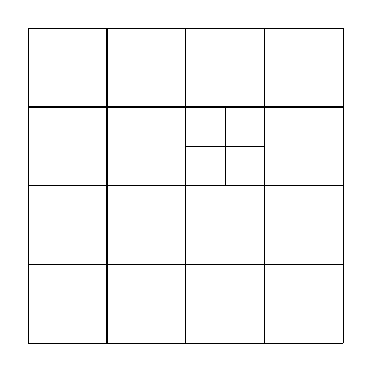
\begin{tikzpicture}[scale = 1]
            \draw[step = 1cm](0,0) grid (4,4); 
            \draw[step = .5cm](2,2) grid (3,3);
        \end{tikzpicture}
    }
    \caption{网格加密形式}
\end{figure}
原因是Basilisk判断到在\ref{fig:exp}$A$处出现了相邻网格层级“越迁”的现象,是故将所涉及的周围网格全部重新加密。
\subsection{网格点插值与平均}
公式\ref{equ:L}表明计算相应数值需要等距网格中心点处的数值,而由于网格之间可能存在一级的错位,则需要插值或平均得到相应位置的拟合数据再进行计算,如图\ref{fig:bili}
\begin{figure}[H]
        \centering
        \includegraphics[width = 0.8\textwidth]{bilinear.png}
        \caption{网格插值与平均计算示意图,截取自\cite{popinet2015quadtree}}
        \label{fig:bili}
\end{figure}
如果要求解目标画圈黑点上的相应$relax$函数值,则需要周边同等级数据点的参与,其中包含并不存在的红色数据点,而想要使用双线性插值求解红色数据点,则需要包围数据点的母网格中心数据,即图中三个黑色点与一个蓝色点。\par
其中蓝色数据点并不存在,需要使用其子网格上四个数据进行平均得到,从而求取所需的红色数据点。获得相应数据后再经由\ref{equ:L}计算目标网格数据值即可。
\printbibliography[heading=bibintoc, title=\ebibname]
\end{document}
